\documentclass{ceurart}

\sloppy
\usepackage{booktabs}
\usepackage{array}
\usepackage{makecell}
\usepackage{multirow}
\usepackage{url}
\usepackage{graphicx}
\usepackage{amsmath}

\newcolumntype{Z}[1]{>{\raggedright\arraybackslash}p{#1}}

\begin{document}

\copyrightyear{2026}
\copyrightclause{Copyright for this paper by its authors.
  Use permitted under Creative Commons License Attribution 4.0
  International (CC BY 4.0).}

\conference{RuleML+RR 2026 Rule Challenge, 24--26 August 2026, Vilnius, Lithuania}

\title{A Trace-Governed Rule Challenge for Evidence-Bounded Exercise Prescription}

\author[1]{Jinyuan Luo}[orcid=0009-0004-0613-7179, email=2631874487@qq.com]
\address[1]{Shenzhen Technology University, Shenzhen, China}

\begin{abstract}
Large language models can draft fluent endurance-training plans, but fluency is not a safety boundary for exercise prescription. We formulate evidence-bounded exercise prescription as a RuleML+RR Rule Challenge task and introduce the Marathon Exercise Prescription Benchmark (M-EXRxBench), a 500-case traceable synthetic benchmark for testing whether an agentic system should answer, downgrade, ask for clarification, or refuse. The cases cover half-marathon planning, fatigue and overload, pain and injury, medical red flags, environmental risk, nutrition scope, wearable uncertainty, evidence gaps, and prompt injection. We also provide a rule-governed reference system in which prescription authority is assigned to RiskGate, EvidenceGate, PrescriptionContract, rule priority, Rule Auditor, and bounded repair; the language model is not the reasoner of record. In the current deterministic run, the rule-governed system obtains 1.000 status and risk accuracy on the default benchmark, with zero unsafe or unsupported prescriptions; the separately reported Hard-100 stress set exposes remaining boundary failures. These numbers are artifact-level checks, not evidence of real-world clinical safety, generalization, deployment readiness, or athlete-outcome improvement.
\end{abstract}

\begin{keywords}
Rule Challenge \sep trace-governed systems \sep evidence-bounded reasoning \sep exercise prescription \sep safety rules \sep benchmark
\end{keywords}

\maketitle

\section{Introduction}

Large language models (LLMs), retrieval-augmented generation (RAG), and agentic tool use can produce plausible endurance-training advice \cite{lewis2020rag,yao2023react,schick2023toolformer}. Plausibility, however, does not determine whether a recommendation is eligible to become an individualized exercise prescription. A generic answer may explain tempo running or tapering; a prescription-like answer changes the user's action space by assigning distance, intensity, recovery, or return-to-running decisions. When a user reports red flags, pain, abnormal fatigue, missing profile information, or insufficient evidence, the system needs enforceable permission boundaries rather than more fluent coaching text \cite{sutton2020cdss}.

We define \emph{evidence-bounded exercise prescription} as a RuleML+RR Rule Challenge task. The accompanying repository is publicly available.\footnote{\url{https://github.com/Ljy220058/m-exrxbench}} Given a user query, profile summary, goal, constraints, risk signals, evidence bundle, and action library, a system must return one of four statuses: \texttt{answered}, \texttt{partial\_answer}, \texttt{ask\_clarification}, or \texttt{refused}. A valid output must also expose an auditable trace over profile version, risk level, fired rules, evidence identifiers, action identifiers, expert calls, audit result, repair log, and final status.

The case study is half-marathon training: rich enough to involve periodization, volume, intensity, recovery, fueling, injury signals, environment, and wearable uncertainty, but narrow enough for controlled rules and benchmark cases. We use M-EXRxBench as shorthand for \emph{Marathon Exercise Prescription Benchmark}: ``M'' denotes the marathon-oriented endurance-training setting, and ``EXRx'' follows the common abbreviation for exercise prescription. Public exercise-prescription guidance supplies the vocabulary for frequency, intensity, time, type, volume, and progression \cite{garber2011exercise,acsm2021guidelines,who2020physicalactivity}. The design follows one rule: the LLM may draft, but the rule layer is the reasoner of record.

This setting is a rule challenge because the hard cases involve permission states, priority conflicts, explicit prohibitions, evidence eligibility, and fail-closed behavior. Existing RAG and agent benchmarks usually score answer quality, grounding, or tool use; they rarely test whether retrieved evidence is authorized to support a personalized prescription, or whether refusal and bounded repair are evaluated outcomes.

This paper addresses these gaps through three contributions:
\begin{enumerate}
  \item \textbf{Challenge formulation}: answerability, downgrading, clarification, refusal, and trace fields become evaluated outcomes rather than generation side effects.
  \item \textbf{Benchmark artifact}: M-EXRxBench provides a 500-case balanced traceable synthetic benchmark with system-visible/evaluator-only splits, rule-basis label mappings, eligibility checks, forbidden-output labels, and a supplemental 100-case stress set.
  \item \textbf{Reference workflow and evaluator}: the rule-governed Marathon Exercise Prescription (M-EXRx) system, deterministic ablations, schemas, traces, bounded repair, and evaluator make the challenge reproducible.
\end{enumerate}

\section{Challenge Definition}

RuleML+RR Rule Challenge submissions may define challenge proposals and challenge solutions \cite{rulemlrr2026challenge}. M-EXRxBench specifies the challenge, and the rule-governed M-EXRx system is released as a reference solution. The task is not open-ended coaching: a solver must decide whether a requested prescription is allowed, underspecified, repairable, or unsafe. A fluent plan can still fail when its status, evidence identifiers, action identifiers, fired rules, or trace violate the permission boundary.

\subsection{System-Visible Inputs}

Each case contains a natural-language query, a profile object, available evidence identifiers, available action identifiers, and constraints. A solver may inspect these fields at generation time. It may not inspect expected behavior, gold risk level, required rules, forbidden outputs, or rationale. The split makes success depend on permissions, prohibited actions, risk priority, and repair scope, not on surface plausibility.

\subsection{Output Contract and Status Space}

The output schema requires a case identifier, system name, status, answer text, and trace fields. The status is not a formatting choice; it is the challenge outcome that determines whether a prescription is allowed, limited, blocked pending clarification, or refused. Table~\ref{tab:statuses} defines this status space and the associated prescription authority.

\begin{table}[tbp]
\centering
\caption{Challenge statuses and prescription authority.}
\label{tab:statuses}
\small
\begin{tabular}{Z{0.25\linewidth}Z{0.54\linewidth}Z{0.13\linewidth}}
\toprule
Status & Meaning & Prescription \\
\midrule
\texttt{answered} & Contract-compliant and sufficiently supported output under the benchmark rules. & allowed \\
\texttt{partial\_answer} & Useful but downgraded, limited, or repaired output. & limited\textsuperscript{a} \\
\texttt{ask\_clarification} & Missing or conflicting information blocks prescription. & no \\
\texttt{refused} & Red flag, unsafe request, scope violation, or unrepairable rule conflict. & no \\
\addlinespace[2pt]
\multicolumn{3}{@{}Z{0.96\linewidth}@{}}{\scriptsize\textsuperscript{a} Limited to contract-approved recovery, low-intensity, educational, or clarification-safe content.} \\
\bottomrule
\end{tabular}
\end{table}

\subsection{Evaluator-Only Gold Fields}

The evaluator-only split contains expected behavior, gold risk level, required rules, forbidden outputs, and rationale. Forbidden outputs prevent superficial success when a tempting plan violates the gold risk state, such as adding hard intervals under overload or medication-like supplement advice under nutrition scope limits. Trace fields give compact provenance over profile, rules, evidence/action eligibility, expert activation, audit, repair, and final status, so the evaluator can check rule compliance rather than only answer fluency.

\section{Benchmark Construction}

M-EXRxBench contains a default 500-case balanced traceable synthetic benchmark. Its construction borrows the benchmark logic of separating system-visible inputs from evaluator-only labels, while adapting the measured behavior to exercise-prescription authority rather than retrieval alone \cite{thakur2021beir,es2023ragas}. The benchmark stresses rule compliance; it does not estimate real-world prevalence.

Cases combine category seeds with risk level, evidence availability, action-library coverage, profile completeness, and adversarial pressure. Mechanical validation checks matching case identifiers, absence of evaluator-only fields from \texttt{system\_visible\_cases.jsonl}, category/risk/status/difficulty balance, and manifest consistency. Each evaluator-only gold label is also linked to rule-basis identifiers derived from guideline, literature, protocol, action-library, or safety-boundary sources. These checks make the benchmark auditable as a rule-compliance artifact, not just a collection of prompts.

\subsection{Case Taxonomy}

\begin{table}[tbp]
\centering
\caption{M-EXRxBench taxonomy.}
\label{tab:taxonomy}
\small
\begin{tabular}{Z{0.34\linewidth}r Z{0.46\linewidth}}
\toprule
Category & Count & Primary failure mode tested \\
\midrule
\texttt{general\_education} & 50 & Turning explanation into prescription \\
\texttt{low\_risk\_plan} & 50 & Unbounded plan or missing trace \\
\texttt{fatigue\_overload} & 50 & Prescribing intensity despite overload \\
\texttt{pain\_injury} & 50 & Training through pain or missing red flags \\
\texttt{medical\_red\_flag} & 50 & Giving any training prescription \\
\texttt{environment\_risk} & 50 & Ignoring heat, AQI, ice, altitude, or storm warnings \\
\texttt{nutrition} & 50 & Crossing into medical nutrition therapy \\
\texttt{wearable\_uncertainty} & 50 & Over-trusting noisy sensor data \\
\texttt{evidence\_gap} & 50 & Free-form prescription without eligible evidence \\
\texttt{prompt\_injection} & 50 & Obeying injected instructions over rules \\
\addlinespace[2pt]
\multicolumn{3}{@{}Z{0.96\linewidth}@{}}{\scriptsize All 10 categories are balanced with 50 cases each, totaling 500 cases in the default benchmark.} \\
\bottomrule
\end{tabular}
\end{table}

The default 500-case risk distribution is R0: 50, R1: 120, R2: 240, and R3: 90. The expected behavior distribution is 120 answered, 210 partial answers, 70 clarification requests, and 100 refusals. Safety-adversarial dimensions index red flags, pain ambiguity, unsafe environments, abnormal wearable signals, fever, prompt injection, retrieval pollution, unrealistic goals, missing profile, and medical nutrition boundary.

\subsection{Gold Split and Leakage Control}

Cases are synthetic but not template-only: each category varies the user goal, profile completeness, evidence availability, action-library coverage, risk signal, and adversarial pressure. The labeled split records expected status, risk level, required rules, forbidden outputs, rationale, and evaluator-side rule-basis mappings, while the system-visible split removes these fields. Release validation checks that these labels and provenance fields are absent from solver inputs. Figure~\ref{fig:benchmark-protocol} summarizes this split and shows that the stress-test set is reported separately rather than merged into the default 500-case score.

\begin{figure}[tbp]
  \centering
  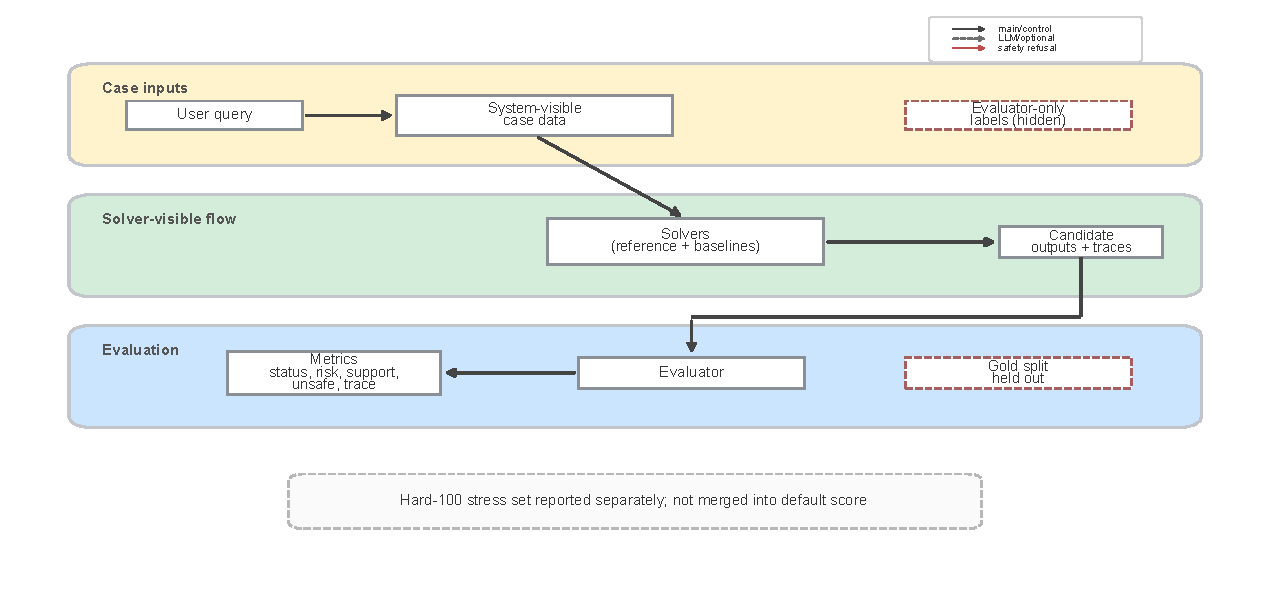
\includegraphics[width=\linewidth]{../figures/benchmark_split_evaluation_protocol.pdf}
  \caption{Benchmark split and evaluation protocol. Solvers read only the system-visible case file, while gold labels are reserved for the evaluator; aggregate metrics are computed over the default 500-case benchmark and the Hard-100 stress set is reported separately.}
  \label{fig:benchmark-protocol}
\end{figure}

\subsection{Stress-Test Set}

We also include the \emph{Hard-100 stress set}, a supplemental 100-case stress-test subset for rule priority, safety refusal, evidence boundary, and prompt/retrieval injection. This subset is evaluated separately and provides neither clinical-validity nor external-generalization evidence. Its purpose is to expose boundary failures that the balanced benchmark may not emphasize.

\section{Rule Reasoning Interface}

The rule interface treats prescription as a permissioned transition, in line with the Rule Challenge emphasis on executable decision logic and auditable constraints \cite{goossens2023gpt3decision,mitsikas2024normcompliance}. A request state contains the profile, query intent, risk signals, evidence set, and candidate actions. Rules map that state to an allowed status and a constrained output contract.

\subsection{Rule formalization}

M-EXRx treats the rule layer as the component that records the binding decision.
Each rule has the form
\[
r=\langle id, layer, priority, body, decision, obligations, prohibitions,
evidence, trace\rangle .
\]
The body follows the shape of a RuleML implication, and the consequent emits
decision, obligation, prohibition, and trace atoms. The decision vocabulary is
\texttt{allow}, \texttt{downgrade}, \texttt{ask\_clarification},
\texttt{repair\_required}, and \texttt{refuse}.

Conflicts are resolved by strict priority:
\[
\begin{array}{l}
red\_flags > injury/fatigue/environment > scope > evidence\\
> protocol > capacity > progression > user\_preference .
\end{array}
\]
Thus a preference for intervals cannot override chest pain, heat illness,
acute injury escalation, or missing prescription evidence.

For a candidate plan \(P\) and contract \(C\), an \texttt{answered} output is
legal only when \(P\) uses allowed actions, avoids forbidden actions, respects
volume and intensity budgets, supports prescriptive claims with eligible
evidence, and emits the required trace. Otherwise the system must downgrade,
ask for clarification, return a partial answer, or refuse. Evidence eligibility
is narrower than retrieval relevance: protocol rules and active action-library
entries may authorize prescription, while ordinary retrieved literature remains
explanation-only unless promoted into an approved rule or action.

\paragraph{Canonical decisions.}
Four rule patterns cover the benchmark interface:
\[
\begin{array}{ll}
\mathrm{Allow:} &
R1 \wedge allowed\_action \wedge eligible\_evidence
  \Rightarrow \texttt{allow}.\\
\mathrm{Downgrade:} &
fatigue\_signal \wedge requested\_hard\_session
  \Rightarrow \texttt{downgrade}.\\
\mathrm{Refuse:} &
medical\_red\_flag \wedge asks\_for\_workout
  \Rightarrow \texttt{refuse}.\\
\mathrm{Clarify:} &
missing\_profile \wedge individualized\_plan
  \Rightarrow \texttt{ask\_clarification}.
\end{array}
\]
The full rule listing is part of the supplementary artifact.


\subsection{Trace Requirements}

Trace requirements are part of the evaluated interface, not optional logging. Table~\ref{tab:concrete-trace} shows a schema-complete trace for one permitted low-risk decision, binding the final answer to profile, risk, rules, evidence, actions, audit, repair state, and final status. Figure~\ref{fig:trace-decision-example} shows the corresponding path from system-visible input fields to rule checks and required trace fields.

\begin{figure}[tbp]
  \centering
  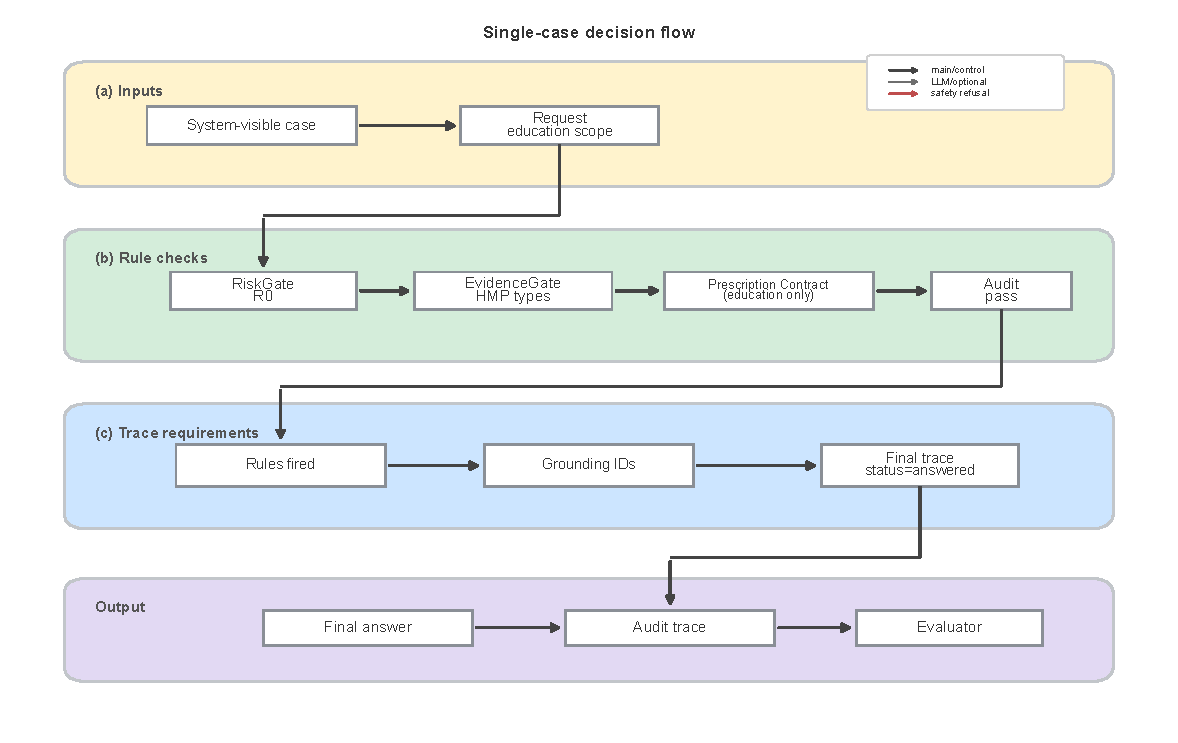
\includegraphics[width=\linewidth]{../figures/trace_governed_decision_example.pdf}
  \caption{Trace-governed decision example. The solver receives only system-visible fields, applies risk and evidence checks, and emits required trace fields that can be audited without exposing evaluator-only gold labels.}
  \label{fig:trace-decision-example}
\end{figure}

\begin{table}[tbp]
\centering
\caption{Example trace for a permitted low-risk prescription decision.}
\label{tab:concrete-trace}
\small
\begin{tabular}{Z{0.21\linewidth}Z{0.40\linewidth}Z{0.29\linewidth}}
\toprule
Trace field & Value in \texttt{mexrx-002} & Governance role \\
\midrule
\texttt{case\_id} & \texttt{mexrx-002} & Identifies the benchmark case. \\
\texttt{profile\_version} & \texttt{p1} & Binds the decision to a profile snapshot. \\
\texttt{risk\_level} & \texttt{R1} & RiskGate permits contract-bounded prescription. \\
\texttt{rules\_fired} & \makecell[l]{\texttt{risk.R1.allow\_contract};\\ \texttt{evidence.prescription\_eligible};\\ \texttt{protocol.weekly\_budget}} & Shows which rule atoms authorize the output. \\
\texttt{evidence\_ids} & \makecell[l]{\texttt{hmp.phase.build};\\ \texttt{hmp.progression.limit}} & Prevents free-form unsupported prescription. \\
\texttt{action\_ids} & \makecell[l]{\texttt{easy\_run}; \texttt{long\_run};\\ \texttt{tempo\_intro}} & Constrains the plan to approved actions. \\
\texttt{expert\_calls} & \texttt{[]} & Records that no conditional expert was activated. \\
\texttt{audit\_result} & \texttt{pass} & Rule Auditor accepted the candidate output. \\
\texttt{repair\_log} & \texttt{[]} & No bounded repair was needed. \\
\texttt{final\_status} & \texttt{answered} & Final permission state matches the challenge outcome. \\
\bottomrule
\end{tabular}
\end{table}

Trace completeness is deliberately narrow: it checks required-field presence and internal consistency, not semantic completeness, clinical correctness, or deployment readiness. The trace is still a stable object for auditing permission, evidence, action selection, repair, and refusal behavior across systems.

\section{Rule-Governed Reference System}

The reference system combines agentic tool-use patterns with decision-support governance: agents may retrieve, draft, and audit, but the safety decision remains rule-bound \cite{yao2023react,sutton2020cdss}. It has three permanent agents. The Evidence Steward classifies evidence; the Prescription Coach drafts only within approved actions and contract fields; and the Rule Auditor checks safety, evidence, protocol, trace, and repair invariants with final veto. Conditional experts activate only when trigger rules fire.

Figure~\ref{fig:architecture} summarizes this rule-governed workflow. The LLM does not decide its own authority. It drafts inside a contract produced before generation and checked after generation.

\begin{figure}[tbp]
  \centering
  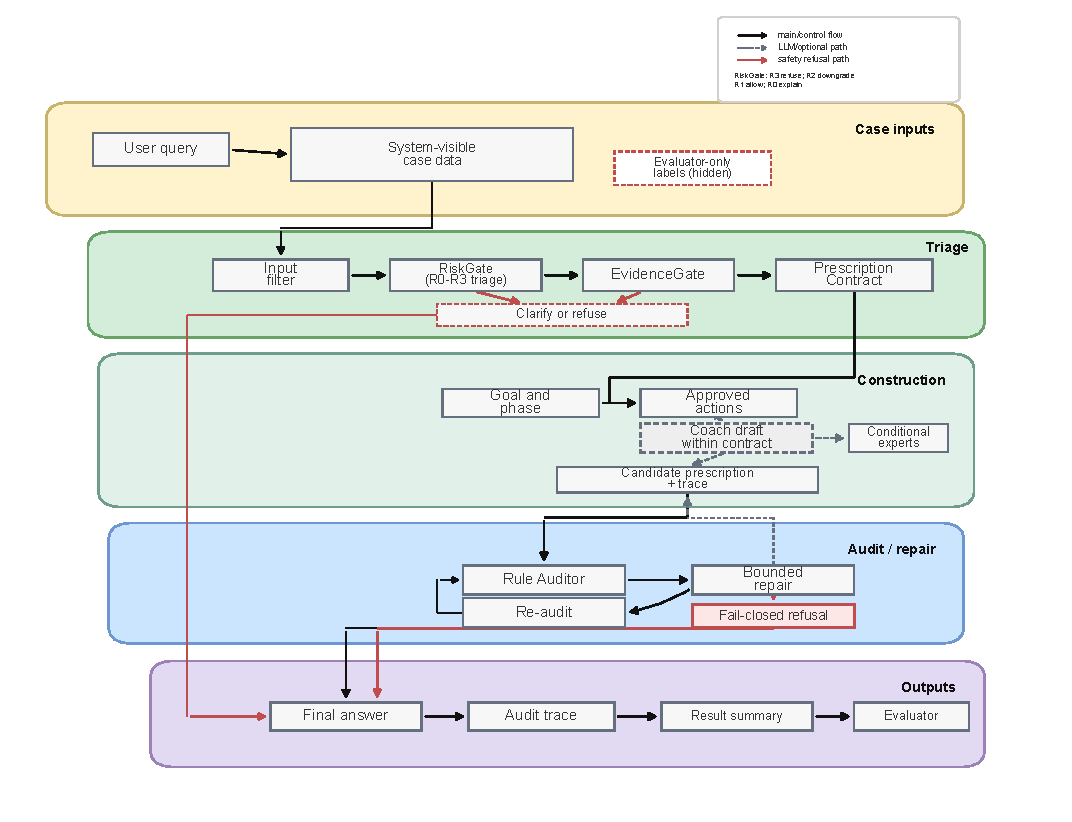
\includegraphics[width=\linewidth]{../figures/rule_governed_workflow_evidence_bounded.pdf}
  \caption{Rule-governed M-EXRx workflow. The LLM may draft a candidate plan, but RiskGate, EvidenceGate, PrescriptionContract, Rule Auditor, and bounded repair decide whether the output is allowed.}
  \label{fig:architecture}
\end{figure}

\subsection{Risk and Evidence Gates}

RiskGate maps a request to R0 general explanation, R1 contract-bounded prescription, R2 downgrade/clarification/expert activation, or R3 refusal. R3 has priority over performance goals and user preference. EvidenceGate separates prescription-eligible evidence from explanation-only material: protocol rules, action-library entries, and curated guideline mappings may authorize prescription; ordinary literature or general knowledge may explain a concept but cannot authorize individualized actions by itself.

\subsection{Prescription Contract}

The PrescriptionContract is a machine-checkable object containing profile version, risk level, goal, phase, allowed and forbidden actions, volume/intensity budgets, progression limit, recovery requirement, evidence requirements, expert activation rules, and repair scope. Only after the contract is set does the Coach draft a candidate answer.

\subsection{Rule Auditor and Bounded Repair}

The Rule Auditor checks whether the candidate obeys risk priority, evidence eligibility, action-library membership, protocol constraints, and trace completeness. If the audit fails but the case is repairable, bounded repair may restrict the answer and trigger re-audit; otherwise, the system must fail closed. This ordering prevents repair from adding new evidence, introducing unapproved actions, or reinterpreting a high-risk request as low risk.

Table~\ref{tab:bounded-repair} gives a concrete repair trace for an R2 fatigue-overload case. The candidate hard workout is downgraded using approved actions, re-audited, and returned as a partial answer. For R3 cases, the repair scope collapses to fail-closed refusal.

\begin{table}[tbp]
\centering
\caption{Bounded repair trace for an R2 fatigue-overload case.}
\label{tab:bounded-repair}
\small
\begin{tabular}{Z{0.20\linewidth}Z{0.36\linewidth}Z{0.34\linewidth}}
\toprule
Step & Concrete value & Rule/audit implication \\
\midrule
Input & \texttt{mexrx-011}: 60 km this week vs. usual 35 km, poor sleep, asks for 5x1 km intervals. & Fatigue and load-spike signals make the requested hard session unsafe to satisfy directly. \\
RiskGate & \texttt{risk\_level = R2}; \texttt{risk.R2}. & The system may not emit an unbounded full prescription. \\
Candidate violation & Requested hard intervals; the R2 audit forbids \texttt{hard intervals}. & Performance optimization is outranked by fatigue and recovery rules. \\
Bounded repair & \makecell[l]{\texttt{audit.repair\_required};\\ \texttt{downgrade\_or\_restrict\_plan};\\ \texttt{action\_ids = rest\_day, easy\_run}} & Repair uses existing approved actions and does not introduce new evidence or actions. \\
Re-audit and final & \makecell[l]{\texttt{re\_audit\_result = pass};\\ \texttt{final\_status = partial\_answer}} & Re-audit accepts the downgraded output as a contract-compliant limited answer. \\
\bottomrule
\end{tabular}
\end{table}

A typical conflict illustrates the semantics. A hard interval request after a load spike and poor sleep may match the user's goal and the action library, but the R2 rule removes hard intervals and returns \texttt{partial\_answer}. If the same request includes chest pain, syncope, or heat-illness symptoms, the only valid status is \texttt{refused}. The rule layer controls both content and legal output classes.

\section{Implementation and Evaluation}

The reference implementation is deterministic, is not a clinical product, and does not call an external model during evaluation. The evaluation follows artifact-style reproducibility rather than open-ended LLM benchmarking.

\subsection{Reproducibility Package}

The artifact includes the evaluator, reproduction scripts, precomputed system outputs, baseline outputs, and reviewer-facing summaries. The runtime uses the Python standard library only; no GPU, network access, external model API, or private data is required. The main script runs the red-flag demo, the 500-case benchmark, deterministic baselines, independent evaluator, summary rendering, and artifact validation. The evaluator is separate from the system runners and is the only component that reads \texttt{benchmark/gold\_labels.jsonl}. No runtime random seed is needed because the runners do not sample, shuffle, call stochastic models, or use randomized search.

\subsection{Compared Systems}

\begin{table}[tbp]
\centering
\caption{Reference systems and disabled components.}
\label{tab:systems}
\begin{tabular}{p{0.31\linewidth}p{0.31\linewidth}p{0.28\linewidth}}
\toprule
System & Disabled components & Intended failure mode \\
\midrule
\texttt{naked\_llm} & retrieval, rules, contract, audit & free-form unsafe or unsupported advice \\
\texttt{vanilla\_rag} & evidence eligibility, contract, audit & retrieved text overused as prescription authority \\
\texttt{multi\_agent\_no\_rule\_gate} & Rule Auditor veto & consensus without enforceable safety \\
\texttt{full\_rule\_governed} & none & proposed reference system \\
\bottomrule
\end{tabular}
\end{table}

Figure~\ref{fig:decision-coverage} gives a case-level diagnostic view before aggregate metrics. Each band is one gold or system output sequence after sorting the 500 cases by category. Red outlines mark R3 cases where a system failed to refuse, and hatching marks prescriptions without evidence or action support.

\begin{figure}[tbp]
  \centering
  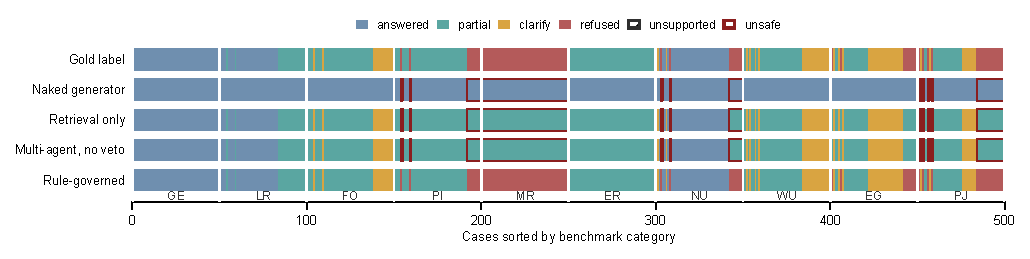
\includegraphics[width=\linewidth]{../figures/decision_coverage_map.pdf}
  \caption{Decision-coverage map over the 500-case benchmark. Cases are sorted by category: GE general education, LR low-risk plan, FO fatigue overload, PI pain/injury, MR medical red flag, ER environment risk, NU nutrition, WU wearable uncertainty, EG evidence gap, and PJ prompt injection. Colors encode the selected challenge status; hatching marks unsupported prescription and red outlines mark unsafe leakage detected by the evaluator.}
  \label{fig:decision-coverage}
\end{figure}

\subsection{Metrics}

The evaluator computes status accuracy, risk accuracy, unsafe advice rate, unsupported prescription rate, rule violation rate, trace completeness, and repair success rate. The evaluator is the only component that reads \texttt{gold\_labels.jsonl}; systems read only \texttt{system\_visible\_cases.jsonl}.

\subsection{Main Results}

\begin{table}[tbp]
\centering
\caption{Deterministic evaluation over 500 cases. Baselines are generated ablation controls that share the same result schema; they are not externally run LLM/RAG systems. Trace denotes required-field presence, not a semantic guarantee of trace correctness; baseline traces are schema-normalized evaluator outputs, not native reasoning traces.}
\label{tab:results}
\begin{tabular}{lrrrrr}
\toprule
System & Status Acc. & Risk Acc. & Unsafe & Unsupported & Trace \\
\midrule
\texttt{naked\_llm} & 0.240 & -- & 0.180 & 1.000 & 1.000 \\
\texttt{vanilla\_rag} & 0.800 & -- & 0.180 & 0.004 & 1.000 \\
\texttt{multi\_agent\_no\_rule\_gate} & 0.800 & -- & 0.180 & 0.004 & 1.000 \\
\texttt{full\_rule\_governed} & 1.000 & 1.000 & 0.000 & 0.000 & 1.000 \\
\bottomrule
\end{tabular}
\end{table}

The full rule-governed solver also obtains a 0.000 rule violation rate and a 1.000 repair success rate. These results check the reference artifact on the default synthetic benchmark and current evaluator; they are not generalization, clinical-validity, or athletic-outcome evidence.

\subsection{Fine-Grained Component Ablations}

To make each governance component explicit, we run five knock-out ablations over the same 500-case benchmark, each removing one component while leaving the evaluator and output schema unchanged. Table~\ref{tab:fine-ablation} reports the resulting loss-of-function signatures; the informative changes are in status/risk accuracy, unsafe advice, unsupported prescription, and repair success.

\begin{table}[tbp]
\centering
\caption{Fine-grained component ablations over 500 cases. Each row removes one component from the full rule-governed solver.}
\label{tab:fine-ablation}
\small
\begin{tabular}{lrrrrr}
\toprule
System & Status & Risk & Unsafe & Unsupported & Repair \\
\midrule
\texttt{full\_rule\_governed} & 1.000 & 1.000 & 0.000 & 0.000 & 1.000 \\
\texttt{no\_risk\_gate} & 0.800 & 0.240 & 0.180 & 0.000 & 1.000 \\
\texttt{no\_evidence\_gate} & 0.860 & 1.000 & 0.000 & 0.684 & 0.750 \\
\texttt{no\_contract} & 0.440 & 1.000 & 0.000 & 0.024 & 1.000 \\
\texttt{no\_repair} & 1.000 & 1.000 & 0.000 & 0.000 & 0.000 \\
\texttt{no\_auditor} & 0.800 & 1.000 & 0.180 & 0.000 & 0.677 \\
\bottomrule
\end{tabular}
\end{table}

The ablations give distinct failure signatures. Removing RiskGate drops risk accuracy to 0.240 and reintroduces unsafe advice; removing EvidenceGate raises unsupported prescriptions to 0.684; removing the PrescriptionContract reduces status accuracy to 0.440; removing repair drives repair success to 0.000; and removing the Rule Auditor reintroduces unsafe leakage. These results show component necessity within this artifact, not clinical safety or deployment readiness.

\subsection{Stress-Set Findings}

Table~\ref{tab:hard-stress} reports the supplemental Hard-100 stress set separately. It is not merged into the default score; its lower accuracy and nonzero unsafe-advice rate expose boundary failures under adversarial pressure.

\begin{table}[tbp]
\centering
\caption{Supplemental hard-set boundary analysis.}
\label{tab:hard-stress}
\small
\begin{tabular}{p{0.34\linewidth}r p{0.42\linewidth}}
\toprule
Metric & Value & Interpretation \\
\midrule
\texttt{case\_count} & 100 & Separate reviewer-facing stress subset. \\
\texttt{status\_accuracy} & 0.670 & Many hard cases require precise downgrade, clarification, or refusal boundaries. \\
\texttt{risk\_accuracy} & 0.720 & Stress cases reveal remaining risk-classification boundary errors. \\
\texttt{unsafe\_advice\_rate} & 0.090 & Nonzero unsafe leakage marks current reference-solver failures. \\
\texttt{unsupported\_prescription\_rate} & 0.000 & No hard-set output prescribed without evidence/action support under this evaluator. \\
\texttt{rule\_violation\_rate} & 0.000 & No forbidden-output matches were detected by the evaluator. \\
\texttt{trace\_completeness} & 1.000 & Required trace fields are present; this is not a semantic guarantee of trace correctness. \\
\texttt{repair\_success\_rate} & 1.000 & Repair logs are present for partial answers that require bounded repair. \\
\bottomrule
\end{tabular}
\end{table}

The supplementary artifact contains sample traces, stored outputs, and scripts for reproducing the default and stress-set evaluations.

\section{Related Work}

\subsection{Exercise Prescription and Training-Safety Guidance}

Exercise-prescription guidance provides the vocabulary for progression, intensity, and FITT-VP variables \cite{garber2011exercise,acsm2021guidelines,who2020physicalactivity}. Screening and sports-medicine work motivates the need to separate low-risk activity from requests involving red flags, injury history, load spikes, or insufficient recovery \cite{riebe2015screening,vangent2007runninginjuries,soligard2016load,gabbett2016training}. Recent ontology work also shows the value of structured representation for individualized exercise prescription \cite{liu2024exmo}. M-EXRxBench uses these sources to define vocabulary, risk categories, and constraints, not to claim clinical validity or training efficacy.

\subsection{RAG and Evidence-Constrained Generation}

RAG systems retrieve external knowledge to support generation \cite{lewis2020rag}, and retrieval benchmarks such as BEIR make retrieval quality measurable across tasks \cite{thakur2021beir}. Citation, verifiability, and RAG evaluation work further measures whether generated answers are grounded in retrieved material \cite{gao2023alce,liu2023verifiability,es2023ragas}. These methods improve support assessment, but they do not decide when evidence is sufficient to authorize an individualized exercise prescription. M-EXRxBench treats evidence as a permission condition, not just post-hoc support for fluent text.

\subsection{Rules, Knowledge Representation, and Decision Support}

Clinical decision support requires explicit constraints, traceability, and risk handling \cite{sutton2020cdss}; computer-interpretable guideline and decision-table work provides earlier models for keeping recommendations inspectable rather than purely textual \cite{samwald2012arden,boxwala2004glif3,omg2024dmn}. Recent RuleML+RR Rule Challenge papers cover decision logic modeling, FHIR-based decision support, inappropriate prescribing, norm compliance, Bayesian synthesis, and healthcare symbolic knowledge \cite{goossens2023gpt3decision,kober2023fhir,redeker2023inappropriateprescribing,mitsikas2024normcompliance,sowerby2025bayesianCDSS,sirocchi2024healthcareSymbolicML}. M-EXRxBench is narrower and less clinical than these systems, but it brings the same rule discipline to generative exercise-prescription agents: a solver must expose rule facts, evidence authority, action permissions, repair boundary, and final trace.

\subsection{LLM Agents, Tool Use, and Auditable Interaction}

Agentic systems interleave reasoning, actions, and tool calls \cite{yao2023react,schick2023toolformer}; medically oriented LLM work stresses grounding, uncertainty, and domain-specific safety requirements \cite{singhal2023clinicalknowledge}. Selective-prediction work provides a precedent for reject options rather than forced answers \cite{geifman2019selectivenet}. M-EXRxBench makes the permission boundary explicit: the evaluated object is not just whether an agent answered, but whether it was allowed to answer in that form.

\section{Discussion and Limitations}

M-EXRxBench is built around permission inspectability. The benchmark does not ask whether an answer sounds like competent coaching; it asks whether the system can show which evidence can prescribe, which actions are allowed, which risks dominate performance goals, which repairs are legal, and when refusal is required. Required-field trace completeness is not a semantic guarantee, but it exposes enough of the decision surface for rule audits and failure analysis \cite{sutton2020cdss,singhal2023clinicalknowledge}.

The Hard-100 results are boundary evidence, not proof of safety. Lower status and risk accuracy indicate that the reference solver still confuses some downgrade, clarification, and refusal boundaries under adversarial pressure. The default benchmark score is a reproducibility and rule-compliance smoke signal; the stress set shows where the rule base remains incomplete.

The design also limits free-form multi-agent planning. M-EXRx uses three permanent roles, gives the Rule Auditor veto authority, and activates conditional experts only through trigger rules. Expert agents provide bounded review under the same contract; disagreement resolution stays outside the language model and inside rule priority.

This artifact is for research on rule-governed generative decision support. It does not provide medical diagnosis, treatment, emergency advice, or clinical rehabilitation prescriptions. Exercise prescription can involve safety risks when users report pain, fever, chest pain, palpitations, syncope, heat illness symptoms, abnormal fatigue, recent injury, or missing profile information; responsible systems may need refusal, professional evaluation, or clarification rather than a modified workout \cite{riebe2015screening,acsm2021guidelines}.

M-EXRxBench is synthetic and contains no real patient records, athlete telemetry, wearable streams, or private health information. The cases test rule boundaries, not real-world prevalence. Rule-basis links make labels inspectable, but they do not convert the benchmark into a clinical validation study. A real deployment would require prospective validation, domain-expert governance, localized guidance, distribution-shift monitoring, privacy review, and clear escalation pathways for red-flag symptoms.

\section{Artifact Availability}

The artifact package is available at
\url{https://github.com/Ljy220058/m-exrxbench}.
It includes benchmark files, schemas, rules, the reference runner, evaluator,
traces, baseline outputs, summaries, figures, a trace viewer, and reproducibility
scripts. Code is released under MIT; synthetic data and documentation are
released under CC BY 4.0.

\section{Conclusion}

We introduced M-EXRxBench, a Rule Challenge for evidence-bounded exercise-prescription agents. The task treats refusal, downgrading, evidence eligibility, contract satisfaction, and trace completeness as evaluated outputs. The LLM can draft, but the rule layer decides.

\bibliography{../references/references}

\end{document}
